% =====================================================================
% TTM4165 Digital Economics — Case Study template (group of 4)
% Compile on Overleaf with pdfLaTeX + Biber (Overleaf does this by default).
% =====================================================================
\documentclass[11pt,a4paper]{article}

% ---------- Guidance switch ------------------------------------------
% Grey guidance text is shown while you write. Set to false before
% submitting and every \guide{...} disappears.
\newif\ifshowguidance
\showguidancetrue
% \showguidancefalse   % <- uncomment before submission

% ---------- Packages -------------------------------------------------
\usepackage[utf8]{inputenc}
\usepackage[T1]{fontenc}
\usepackage[english]{babel}
\usepackage{lmodern}
\usepackage[margin=2.5cm]{geometry}
\usepackage{setspace}\onehalfspacing
\usepackage{parskip}
\usepackage{graphicx}
\usepackage{booktabs}
\usepackage{tabularx}
\usepackage{array}
\usepackage{enumitem}
\usepackage{xcolor}
\usepackage{amsmath,amssymb}
\usepackage{float}
\usepackage{caption}
\usepackage{pdflscape}
\usepackage{pdfpages}   % for including the NTNU AI declaration form
\usepackage{tikz}
\usetikzlibrary{positioning,arrows.meta,shapes}
\usepackage[style=ieee,backend=biber]{biblatex}  % numbered citations [1], [2, p. 5]
\addbibresource{references.bib}
\usepackage[hidelinks]{hyperref}

% ---------- Helper commands -----------------------------------------
\definecolor{guidegray}{gray}{0.45}
\newcommand{\guide}[1]{\ifshowguidance{\color{guidegray}\itshape #1\par}\fi}
\newcommand{\fillin}[1]{\textbf{[#1]}}
% Placeholder box for a figure you have not made yet.
% Replace with \includegraphics[width=\linewidth]{figures/yourfile.png}
\newcommand{\placeholder}[2][6cm]{%
  \fbox{\parbox[c][#1][c]{0.95\linewidth}{\centering\color{guidegray}#2}}}
\newcolumntype{Y}{>{\raggedright\arraybackslash}X}
\setlength{\emergencystretch}{3em}   % avoids lines running into the margin

% ---------- Title info ----------------------------------------------
\newcommand{\alliancename}{S3NS}
\newcommand{\groupnumber}{106}

% NTNU logo above the title (file uploaded to the figures folder)
\title{
\includegraphics[width=0.45\linewidth]{figures/NTNU hovedlogo - farger - bredde.png}\\[1.5cm]
Sovereignty on Borrowed Technology:\\[4pt]
\large Ecosystem, Platform and Security Economics of \alliancename,\\
the Thales--Google Cloud Trusted-Cloud Alliance}
\author{TTM4165 Digital Economics, Group \groupnumber\\[6pt]
% Remove the names below for the anonymous 28 October peer-review version
\normalsize
\begin{tabular}{c}
Sondre Mathias Nedreberg Burud\\
Even Baanrud\\
Anders Alexander H{\ae}rum Eltoft\\
Arne Skogan
\end{tabular}}
\date{NTNU, Autumn 2026}

\setcounter{tocdepth}{3}   % show tasks and their parts in the contents

\begin{document}
\maketitle

\guide{Target for a group of 4: about 5,000 words (4,500–5,500 is within
$\pm$10\%) and at least 6 peer-reviewed sources. Figures, tables, references
and appendices do not count. Delete this guidance before submitting by
switching \texttt{\textbackslash showguidancefalse} in main.tex.}
\IfFileExists{figures/AI-declaration-signed.pdf}{%
  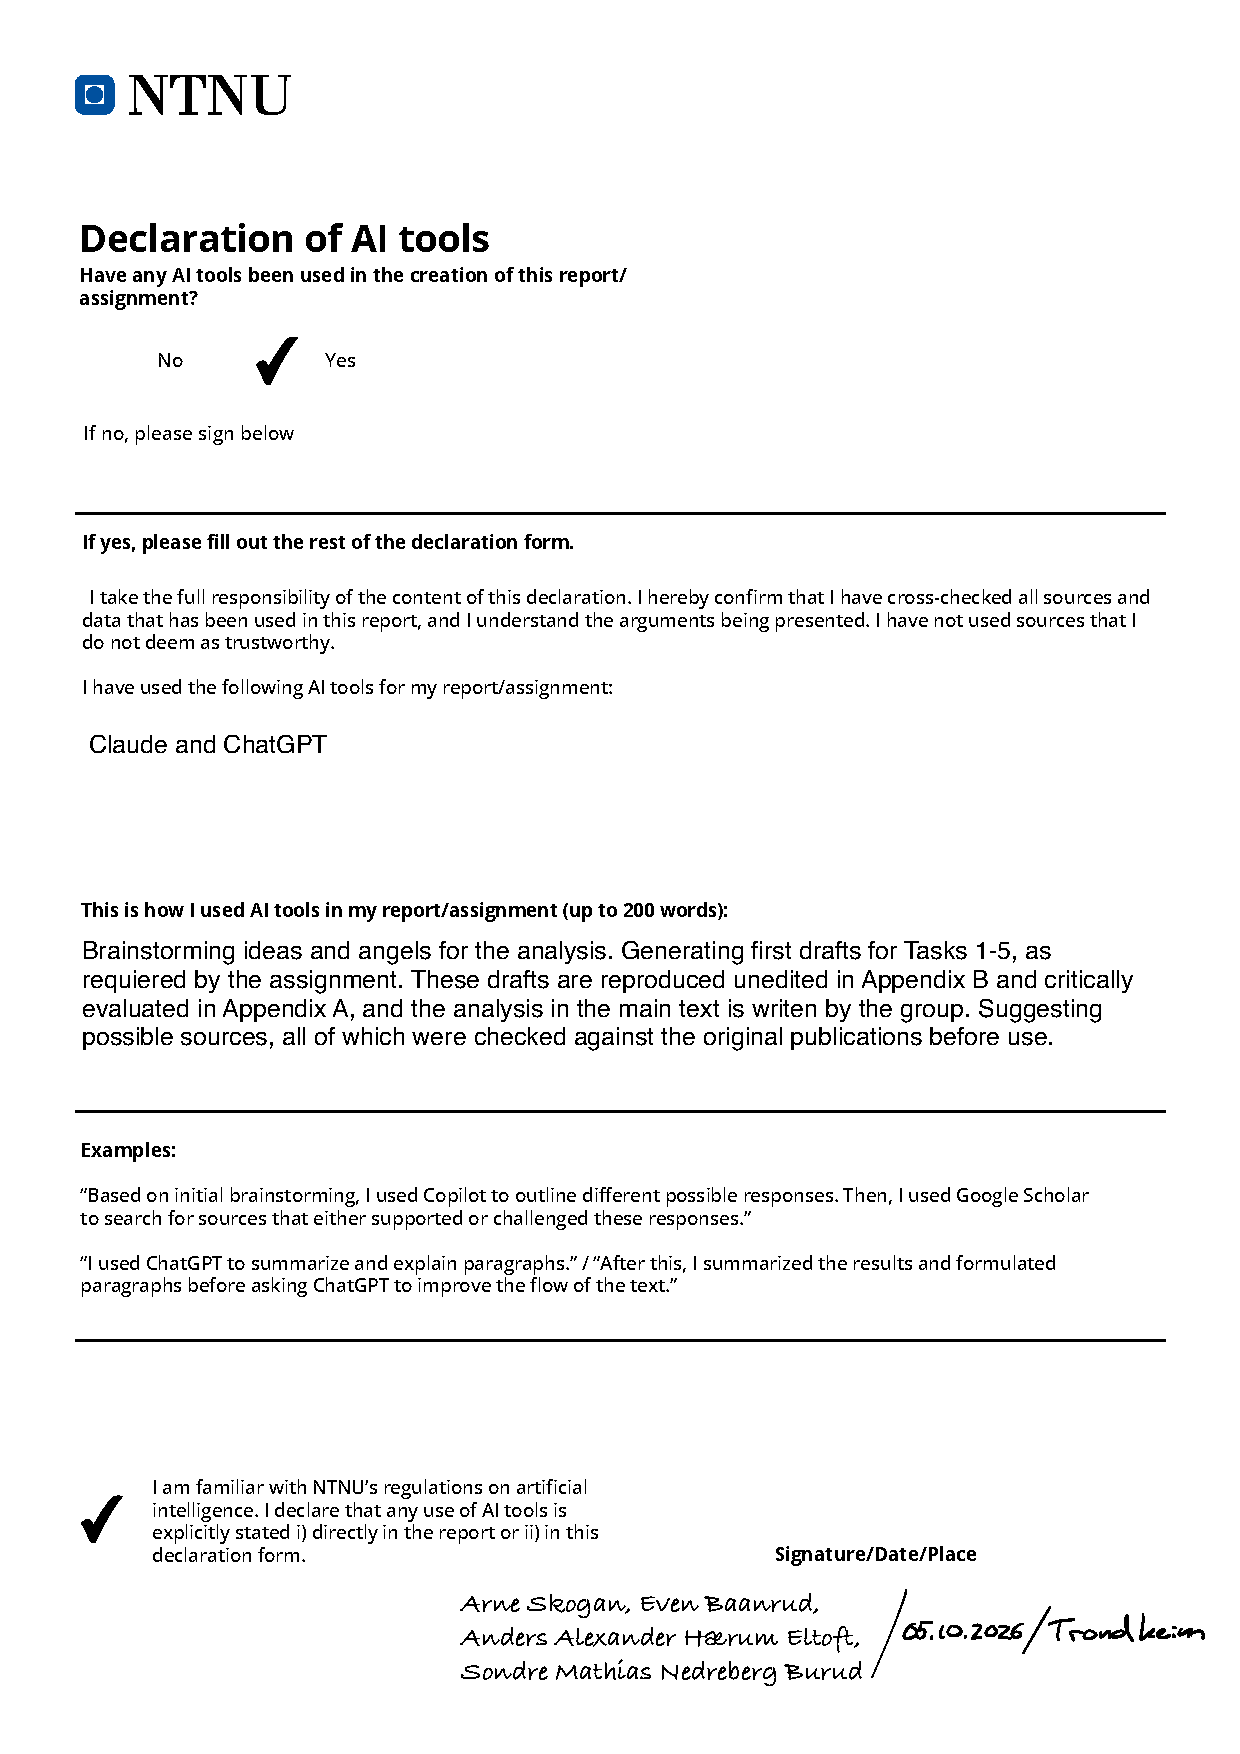
\includepdf[pages=-,pagecommand={\thispagestyle{plain}}]{figures/AI-declaration-signed.pdf}%
}{%
  \guide{Signed form not found: upload it as figures/AI-declaration-signed.pdf.}%
}
\tableofcontents
\newpage

% Planning page — only visible while guidance is on.
\ifshowguidance
\section*{Planning page (hidden when guidance is off)}

\subsection*{Word budget and owners}
\begin{tabularx}{\linewidth}{Yrl}
\toprule
Section & Target words & Owner \\
\midrule
1. Introduction & 400 & Arne \\
Task 1 Business Ecosystems & 800 & Arne \\
Task 2 Network Effects \& Path Dependency & 800 & [name] \\
Task 3 Multisided Platform Mapping & 850 & [name] \\
Task 4 Cybersecurity Economics & 900 & [name] \\
Task 5 Business Model Structure & 800 & [name] \\
3. Conclusion & 450 & [name] \\
\midrule
Total & 5,000 & \\
\bottomrule
\end{tabularx}

\subsection*{Submission checklist}
\begin{itemize}[label=$\square$]
  \item At least 6 peer-reviewed sources (the anchor article and company pages do not count)
  \item Every AI fact and reference checked against a real source
  \item Appendix B holds raw, unedited AI text, max 400 words per task
  \item Appendix A has a critique for all 5 tasks, each naming a course concept
  \item Closing Group Reflection (250--400 words) placed after the appendices
  \item Full 9-block Business Model Canvas + Stakeholder Relationship Model figures
  \item Cybersecurity cost and loss table completed in the main text
  \item NTNU AI declaration form filled in and statement added
  \item Written in English; the alliance, not one company, is the unit of analysis
  \item Names removed for the 28 October peer-review PDF
\end{itemize}
\newpage
\fi

\section{Introduction}
\label{sec:intro}
Cloud computing has become core infrastructure for public administrations and critical sections, but US is the main supplier of the most advanced cloud technology. The US CLOUD Act allows US authorities to demand data from American cloud providers, even when the data is stored outside the United States \parencite{doj2019cloudact}. For European governments handling sensitive data, this creates a conflict between technological capability and control. S3NS was created as a French answer to this problem. It is a company under French law, fully owned by Thales, that runs a trusted cloud based on Google Cloud technology \parencite{s3ns2025premi3ns}.

S3NS describes itself as an alliance between Thales, the French leader in
cybersecurity in Europe, and Google Cloud.
The two partners play different roles. S3NS is a French-law company fully
controlled by Thales, which runs the service in France, while Google Cloud
supplies the underlying technology, including Compute Engine, Cloud Storage,
Cloud SQL, Google Kubernetes Engine and BigQuery.
Every Google technology update is first received in a quarantine zone, where
S3NS analyses and validates it before it is deployed in an environment
administered only by S3NS \parencite{s3ns2025premi3ns}. Google therefore holds
no control over the operation, yet the service cannot function without its
technology. The resulting offering, PREMI3NS, obtained the SecNumCloud 3.2
qualification from the French cybersecurity agency ANSSI in December 2025, and
is used by around thirty early customers, including MGEN, Matmut, Club Med and
Birdz, a Veolia subsidiary. EDF has also announced that it has selected S3NS
\parencite{s3ns2025premi3ns}.

Demand for such services is shaped by regulation. French rules require
sensitive state data hosted with external providers to use SecNumCloud-qualified
services, a principle that began as government cloud policy and was written into
law through the SREN law, with implementing rules adopted in 2026
\parencite{decretsren2026}. S3NS competes with Bleu, a trusted cloud
built by Orange and Capgemini on Microsoft technology \parencite{lemagit2023usf},
and with independent French providers such as OVHcloud. Its ecosystem of
software vendors is still at an early stage \parencite{futurum2026}. The case
therefore raises a central tension: S3NS promises sovereignty, yet depends on a
partner whose technology it cannot replace.

This report asks how the division of roles between Thales and Google shapes
ecosystem dependencies, lock-in, platform pricing, security incentives and value
capture in S3NS. Section~\ref{sec:task1} to Section~\ref{sec:task5} analyse
these questions using the frameworks of \textcite{overby2021} and the course,
and Section~\ref{sec:conclusion} concludes. AI use follows the course
requirements and is documented in Appendices~A and~B.


\section{Analysis}
\subsection{Task 1: Business Ecosystems}
\label{sec:task1}

A business ecosystem is a community of firms that ``coevolve capabilities
around a new innovation'', working both cooperatively and competitively
\parencite[p.~46]{overby2021}. In the digital economy, it describes the
relations and dependencies between digital services, infrastructures, markets
and authorities \parencite[p.~48]{overby2021}. Following \textcite{adner2017},
we start from the value proposition rather than from one firm: cloud services
built on Google technology, run under French control and approved for
sensitive data. The ecosystem consists of the actors that must work together
for this proposition to hold.

Figure~\ref{fig:ecosystem} maps this ecosystem. The blue box is the alliance.
Inside it, Thales owns and controls S3NS, shown by the plain line between them.
S3NS runs PREMI3NS in France, while Google Cloud supplies the underlying
technology, such as computing, storage and data analytics
\parencite{s3ns2025premi3ns}. The grey boxes below are the direct stakeholders.
Client institutions are the customers: around thirty early users, among them
MGEN, Matmut, Club Med and Birdz, while EDF has announced that it has selected
S3NS and Thales itself is a user \parencite{s3ns2025premi3ns}. ANSSI, the
French cybersecurity agency, granted the SecNumCloud qualification in December
2025, which decides whether the offer can host sensitive data at all
\parencite{s3ns2025premi3ns}. Complementors are consultancies, integrators and
software vendors that help clients move to the platform and offer their own
solutions on it \parencite{s3nsecosystem}. The best-known example is SAP, which
has agreed to run its cloud ERP on PREMI3NS \parencite{thalessap2026}.

The orange boxes are indirect stakeholders, which shape the ecosystem without
trading on it. Their influence is shown with dashed arrows. The French state and
US authorities both point at the alliance, because their laws set the
conditions it works under. Under the SREN law and its 2026 decree,
administrations holding particularly sensitive data must use a cloud service
qualified by ANSSI or certified at EU level \parencite{decretsren2026}. The US
CLOUD Act lets US authorities demand data from US providers even when it is
stored abroad \parencite{doj2019cloudact}, which is the reason a
French-controlled offer is needed in the first place. Competitors such as Bleu,
built by Orange and Capgemini on Microsoft technology \parencite{lemagit2023usf},
are linked to the alliance by a two-way dashed arrow, since competition affects
both sides. End users point to the client institutions rather than to the
alliance, because they reach the platform only through the institutions that
hold their data. As \textcite[p.~58]{overby2021} stress, authorities and
consumers are easy to overlook but can decide a firm's survival.

\begin{figure}[htbp]
    \centering
    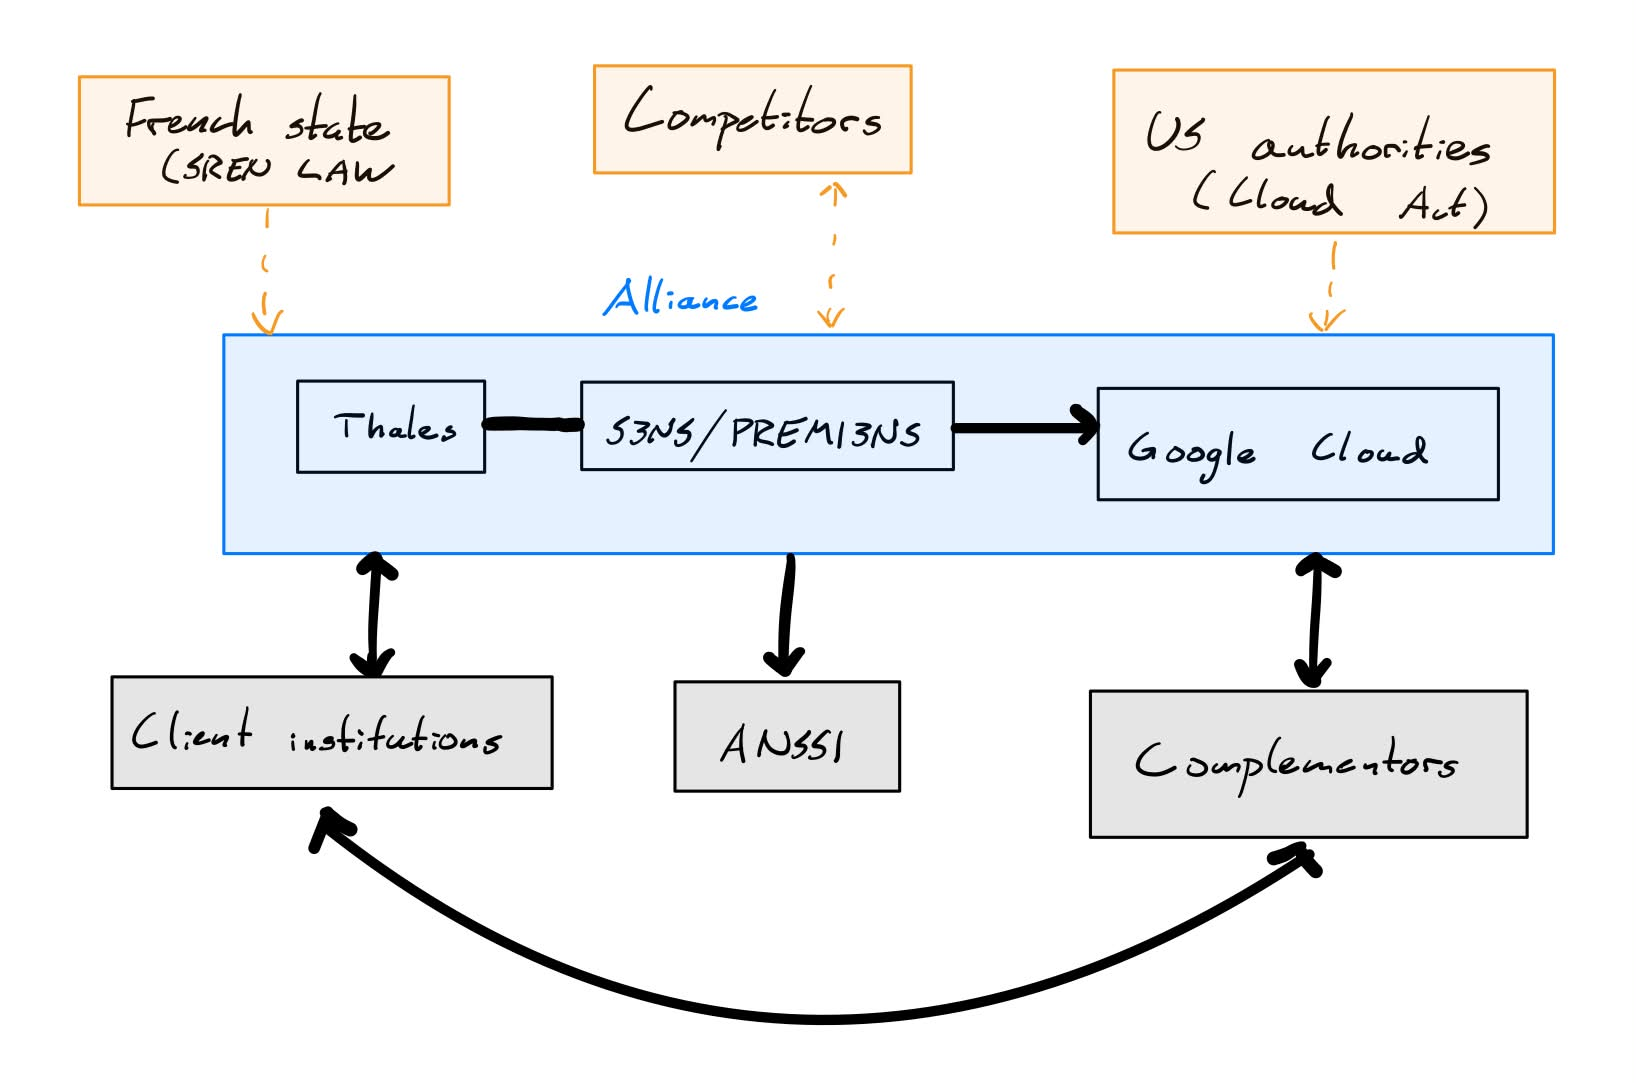
\includegraphics[width=0.85\linewidth]{figures/ecosystem.jpg}
    \caption{Business ecosystem of S3NS. The blue box is the alliance, grey
    boxes are direct stakeholders and orange boxes indirect stakeholders. An
    arrow from A to B means that A depends on B, and a double arrow means mutual
    dependency (notation after \textcite[p.~49]{overby2021}). Dashed arrows show
    indirect influence through law, competition or, for end users, through the
    client institutions. The plain line between Thales and S3NS marks ownership
    and control.}
    \label{fig:ecosystem}
\end{figure}

\subsubsection{Critical relationships and dependencies}

Following the notation of \textcite[p.~49]{overby2021}, a single arrow in
Figure~\ref{fig:ecosystem} shows one-way dependency and a double arrow mutual
dependency. Three of these links are critical.

The first is the single arrow from S3NS to Google Cloud inside the alliance
box. S3NS depends on Google, but Google does not depend on S3NS, so the most
important dependency lies inside the alliance itself. Every Google update first
enters a quarantine zone, where S3NS checks and approves it before it is
deployed in an environment that only S3NS runs \parencite{s3ns2025premi3ns}.
This link carries both the value of the offer, modern cloud services, and its
main risk. Google's technology is closely tied to the service and has no ready
substitute; in course terms it is co-specialised and has low fungibility
\parencite[slide~30]{windekilde2026ecosystem}. S3NS could not switch provider
without rebuilding its service, and clients inherit this dependency through
S3NS, since their systems are built on Google-based services.

The second is the single arrow from the alliance down to ANSSI. The alliance
depends on the qualification, while ANSSI does not depend on the alliance.
This dependency is about regulation rather than technology, but it is just as
critical: without the qualification, the demand created by the SREN law
disappears.

The third is the curved double arrow between client institutions and
complementors. Clients can only move their systems if the software they need
is available on the platform, and vendors only qualify their software if there
are enough clients to sell to. This is why the SAP agreement matters
\parencite{thalessap2026}. The alliance is linked to both groups by double
arrows as well, since it needs their custom and contributions as much as they
need the platform.

\subsubsection{Complementarities}

The partners bring what the other lacks. Google brings technology it has
already built at global scale, while Thales brings French ownership, security
expertise and control. By using Google as its cloud provider, S3NS can offer a
full service without building all the technology itself
\parencite[p.~54]{overby2021}. The complementarity is \emph{unilateral}: S3NS
needs Google's technology to work, but Google's business does not need S3NS
\parencite[p.~114]{overby2021}. This matches the book's example of Skype and
Internet service providers, where Skype needs the providers but not the other
way round \parencite[p.~115]{overby2021}.

PREMI3NS also complements the software of the vendors. For a regulated client,
the platform is worth little unless the applications it needs can run there,
and the software is worth more when it can run inside a qualified cloud. The
complementarity is \emph{supermodular}, meaning that more of one makes the
other more valuable: more qualified software makes PREMI3NS more attractive,
and more PREMI3NS customers make it more worthwhile for vendors to qualify
their software \parencite[slides~27--28]{windekilde2026ecosystem}. This part of
the ecosystem is still small, as the vendor model on PREMI3NS is described as
being at an early stage \parencite{futurum2026}.

\subsubsection{How the alliance changes roles, incentives and influence}

The alliance changes the position of each main actor compared with acting
alone, which is why Thales and Google are drawn inside one box in
Figure~\ref{fig:ecosystem}. Google goes from being a foreign supplier, and a
competitor through its own public cloud, to a technology partner. It reaches
regulated French customers it could not serve directly, but gives up control of
the operation to S3NS. Thales goes from security specialist to cloud owner and
operator, and is also a key customer, both on PREMI3NS and as SAP's first
customer on the platform \parencite{thalessap2026}. The French state goes from
buyer to market creator, since its rules create the demand the alliance serves
\parencite{decretsren2026}. The partners' incentives are not fully aligned:
Thales must guarantee independence, while Google gains from wider use of its
technology, including by repeating the model in Germany
\parencite{thalesgoogle2026}. Influence in the ecosystem therefore rests on a
paradox. Thales holds formal control, but Google holds the technology the whole
ecosystem depends on.
\subsection{Task 2: Network Effects and Path Dependency}
\label{sec:task2}

% \guide{About 800 words. Course basis: Chapters 9 and 11. Does the platform get
% more valuable as users, institutions, agencies, data sources or complementary
% services join? Separate real network effects from plain economies of scale.
% Then discuss path dependency, lock-in, switching costs and tipping.}

This section asks whether PREMI3NS becomes more valuable as more agencies, institutions, and complementary services join, and how early choices shape later ones. We believe that the majority of the alliances' advantage is supply-side economies of scale rather than network effects, that lock-in is nevertheless strong and runs on two levels: from agency to S3NS and from S3NS to Google (Section~\ref{sec:ValueGrowth}), and that the market is therefore likely to see lock-in without tipping (Section~\ref{sec:PathDependency}).  

\subsubsection{Value growth}
\label{sec:ValueGrowth}

\textcite[p.~124]{overby2021} separates supply-side economies of scale from network effects. In economies of scale, size lowers the cost of production; in network effects, the size raises the value each user gets. Most of PREMI3NS' advantage is on the supply side. Google has already paid to develop Compute Engine, Kubernetes Engine, Cloud SQL, and BigQuery and spreads the cost over its global customer base. S3NS offers these services without building them \parencite{s3ns2025premi3ns}. Each new client lowers the average cost, and Thales is reusing the "identical technology and operating model" for a German region \parencite{thalesgoogle2026}. None of this makes the platform more valuable to one agency because another agency has joined. It is scale, not a network effect. 

Real network effects exist, but they are mostly indirect and cross-side \parencite[pp.~135--136]{overby2021}. More SecNumCloud clients make it worthwhile for software vendors to certify on PREMI3NS, and each certified application makes the platform more useful to clients. Because PREMI3NS exposes Google Cloud APIs, it also inherits Google's global pool of skills and tools. That network belongs to Google, not the alliance. Named reference clients such as EDF, MGEN, and Veolia \parencite{s3ns2025premi3ns} create a bandwagon effect \parencite[p.~135]{overby2021} that lowers the next buyer's perceived risk. Direct same-side effects between agencies are weak. We found no evidence that agencies exchange data through the platform, so for core hosting it behaves as a Sarnoff network, where users do not benefit from each other \parencite[pp.~137--138]{overby2021}.

The data network effects that power Google Search \parencite[p.~135]{overby2021} are absent by design, since sovereignty rules keep client data from improving Google's services. Lastly, there is a negative network effect. All clients share one legitimacy base, so a single incident or an adverse ruling on extraterritorial law would devalue the platform for all clients (at once). 


\subsubsection{Path dependency and lock-in}
\label{sec:PathDependency}

Path dependence means that where a market ends up depends on early adopters, network effects, and external events \parencite[p.~167]{overby2021}, and it may ``cause strong vendor lock-in'' \parencite[p.~172]{overby2021}. For S3NS, this means that an agency's initial decision to adopt Google based technology through PREMI3NS shapes and increasingly narrows its future options. For S3NS, lock-in comes mainly from switching costs meaning that customers cannot easily move without being subdued to monetary costs, legal constraints, and technical incompatibilities.

For a client agency, some mechanisms drive this lock-in to the alliance's Google-based platform:

\begin{itemize}
    \item \textbf{Data accumulation.} Datasets in BigQuery and managed databases grow year by year. Moving them is costly. \textcite{oparamartins2016} highlight that data portability remains one of the biggest issues facing cloud adoption.

    \item \textbf{Standards.} Virtual machines and Kubernetes follow open standards and are fairly portable. Managed data services, identity and security configuration rely on proprietary Google APIs. As in the VHS--Betamax case \parencite[pp.~168--169]{overby2021}, incompatible standards make the first choice hard to undo.

    \item \textbf{Sunk costs.} Migration projects and re-accreditation are irrecoverable.     

    \item \textbf{Learning effects.} Staff are trained and certified on Google Cloud, and procedures are built around its tools \parencite[p.~181]{overby2021}.
\end{itemize}

The lock-in works on two levels. The agency depends on S3NS, and S3NS depends on Google for all its technology. What the agency is really tied to is therefore Google's technology, so leaving would mean rebuilding its systems on a different platform. \textcite{overby2021} note that the outcome of a path-dependent market is not always the best one. Agencies accept this risk because they get access to advanced cloud services that they could not easily build themselves. 


\subsubsection{Tipping and winner-takes-all}
\label{sec:Tipping}

Hypothetically, positive feedback can lead to so called "winner takes all markets", meaning that the strong gets stronger and the weak gets weaker \parencite[pp.~130, 168]{overby2021}. Full tipping to S3NS is nevertheless unlikely. 

First, the feedback is weak because same-side network effects are weak (Section~\ref{sec:ValueGrowth}). Second, large institutions use several clouds, and public procurement favours multi supplier frameworks. The textbook shows that when churn between providers is balanced, as in the mobile market, market shares stay stable, and only net churn towards one supplier leads to takeover \parencite[pp.~169--170]{overby2021}. Third, \textcite[pp.~125--126]{arthur1989} shows that when increasing returns are bounded, the market can remain shared. Demand is also split between sovereign offers tied to different hyperscalers (Bleu with Microsoft, S3NS with Google, and independents such as OVHcloud).

The likely outcome is therefore lock-in without tipping: strong for each client, weak across the market. Any winner-takes-all dynamic sits upstream, in which hyperscalers technology becomes the template for European sovereign cloud. The replication of the S3NS model in Germany (see Section~\ref{sec:ValueGrowth}) shows that this contest has started.

\begin{table}[ht]
\centering
\small
\caption{Economies of scale versus network effects on PREMI3NS (classification after \textcite[ch.~9]{overby2021})}
\label{tab:task2}
\begin{tabularx}{\linewidth}{Yllll}
\toprule
\textbf{Mechanism} & \textbf{Type} & \textbf{Direct/indirect} & \textbf{Side} & \textbf{Strength} \\
\midrule
Google spreads its development costs & Economies of scale & -- & -- & High \\
S3NS spreads its fixed costs         & Economies of scale & -- & -- & High \\
\addlinespace
Clients attract software vendors     & Network effect (+) & Indirect & Cross-side & Medium \\
Compatibility with Google Cloud      & Network effect (+) & Indirect & Cross-side & High \\
Well-known reference clients         & Bandwagon (+)      & Indirect & Same-side  & Medium \\
Agencies sharing data                & Network effect (+) & Direct   & Same-side  & Low \\
Client data improving the service    & Data network effect & Indirect & --        & None \\
Shared reputation risk               & Network effect ($-$) & Indirect & Same-side & Latent \\
\bottomrule
\end{tabularx}
\end{table}
\section{Task 3: Multisided Platform Mapping}
\label{sec:task3}





\subsection{Is it really a platform?}


A MSP is a multisided platform that lets two or more distinct groups interact directly, and each group is affiliated with the platform (Hagiu \& Wright, 2015). This test is important for S3NS. The core PREMI3NS looks like a pipeline. S3NS licences Google Cloud Technology, runs it in France under French control and sells capacity to clients. If that were S3NS would be a sovereign reseller, not a platform. 

We argue that PREMI3NS is a hybrid. The pipline part bring in the most of the revenue, but there is a platform laywe on top of it. S3NS presents its offer as an ecosystem where service partners help clients migrate, and independent software vendores, ISVs ass their own solutions on top of the cloud (S3NS, n.d-a). The clearest example is SAP. In 2026 SAP agreed to run its RISE private cloud ERP on PREMI3NS, with commercial availability planned for the second part of 2026 (Thales, 2026a). SAP joins to reach regulated clients it could not otherwise serve, and clients join partly because software like SAP is available inside the trusted perimeter. The value each group gets depends on how many members the other group has. That is the defining feature of MSP (Rochet \& Tirole, 2003; {\0}verby \& Audestad, 2021)}.

Two actors oftenly are wrongly treated as platform sides. Google for instance is not a side. It only supplies the technology to the aliances and is paid for that, but google do not transact with clients through the platform. ANSSI isnt a side either, it only sets the rules that decide who may enter the trusted perimeter at all. Both shape the platform from outside the market it creates. 

\subsubsection{The sides}

\textbf{Side 1: Client institutions.} This side is divided into two groups with their own need. The first is French state administration. When they host sensitive data with an external cloud provider, they must use a SecNumCloud qualified service. That rules started off as the government's "cloud au centre" doctrine and was written into law through the 2024 SREN law, with implementing rules adopted in 2026 (Acteurs Publics, 2026; ANSSI, n.d.). The second group is are large companies in regulated sectors. Around ~30 early adopters tested the PREMI3NS before qualification, and EDF and Thales itself are name users (S3NS, 2025). For these firms, trusted cloud is a strategic choice and not a legal duty. Both groups face high switching costs once they have migrated.

\textbf{Side 2: Complementators}. These are ISVs, SaaS providers and service partners (integrator and consultancies). They must have invest to port to qualify their products, and most can also offer them on competing trusted clouds, so they multi-home. An industry analysis describes the ISV model on PREMI3NS as still at an early age (Futurm Group, 2026). This means the platform does not yet have a large complementor side, which is exactly the chicken-and-egg problem MSP theory describes.


\begin{figure}[H]
    \centering
    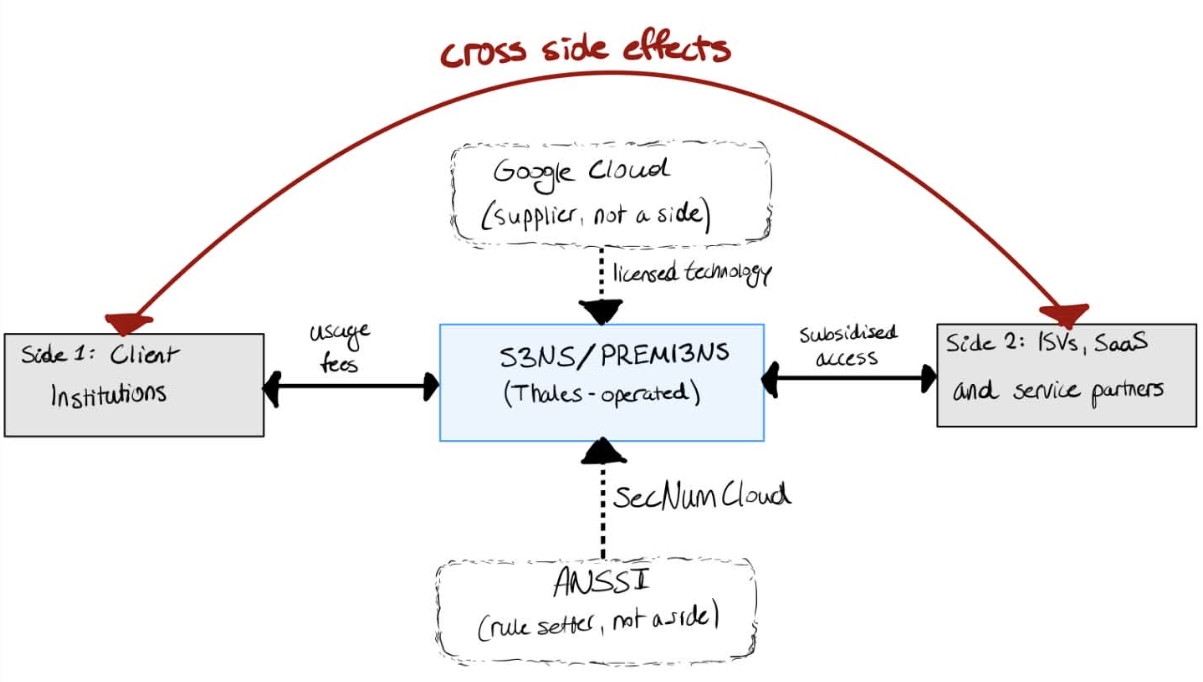
\includegraphics[width=0.90\linewidth]{55555.png}
    \caption{Multisided Platform Map of PREMI3NS. Solid lines are platform sides, dashed lines are suppliers and regulators outside the platform market}
    \label{fig:msp}
\end{figure}

\subsubsection{Cross-side and same-side effects}

The table ~\ref{tab:effects} summarises the effects. The strongest effect runs from the clients to the vendors. Every new regulated client makes the market for SecNumCloud ready software larger and before the qualification this market barely existed. The effect from vendors to the clients is positive but weaker. A client can only move a workload if the software it needs is available, as the SAP case shows for the ERP systems. However, many clients build their own applications directly on the infrastructure, and the Google compatibility means familiar tools are already there. 

The same side effects are weak. Among the clients, early adopters create reference cases and experience that others copy. As the section~3.2 argues for, this is mostly a learning effect and not a true network effect. A ministry does not gain directly because another ministry join. Among vendors, the same-side effect is mostly negative, since they compete for the same small group of clients. 


\begin{table}[h]
\centering
\begin{tabular}{|p{3.3cm}|p{1.4cm}|p{8.3cm}|}
\hline
\textbf{Effect} & \textbf{Strength} & \textbf{Reason} \\ \hline
Clients $\rightarrow$ Vendors & High & New regulated clients open a market that vendors cannot otherwise reach. \\ \hline
Vendors $\rightarrow$ Clients & Medium & More workload can migrate, but many clients build their own applications \\ \hline
Client $\leftrightarrow$ Client & Low (+) & Learning and reference cases, not direct network value \\ \hline
Vendor $\leftrightarrow$ Vendor & Low ($-$) & Competition for the same clients, some shared skills and tools \\ \hline
\end{tabular}
\caption{Cross-side and same-side effects on PREMI3NS (qualitative assessments)}
\label{tab:effects}
\end{table}

\subsubsection{Pricing Architecture}

MSP Theory states that the platform should subsidise the side that is more price sensitive and creates more value for the other side, and it should charge the side whose demand is less elastic (Rochet \& Tirole, 2006; Parker \& Van Alstyne, 2005). A new platform must also get one side on board first to solve the chicken-egg problem (Caillud \& Jullien, 2003). 

The client side is partly documented. S3NS published a catalouge price list in euros. Each service is billed per unit used, for instance per vCPU hour or per gigabyte per month. Many serivces offer a free usage tier, and clients who commit for one or three years get lower unit prices  (S3NS, n.d.-b). For a standard C3 compute core, the one-year price is about 28\% lower and the three-year price about 46\% lower than the pay-as-you-go price. This confirms that the clients are the money side. It also shows a pricing tool that matters for Section~3.2. The commitment discount trades a lower-price today for a longer tie to the platform, so it strengthens lock-in. Clients with sensitve data accept this because the law and the small number of qualified providers make their demand less price elastic. Private firms have more choice, and negotiated commitments let S3NS offer them a lower effective price than state buyers who have to use a qualified cloud. 

the complementor side is not documentes, so we build it from theory. Since the ISV part is still small (Futurm Group, 2026) and vendors multi-home, they should be subsidised through low or zero platform fees, technical help with porting and support toward qualification (A2). The SAP deal shows another kind of subsidy. Thales, one of the alliance partners, became the first customer of SAP on PREMI3NS (Thales, 2026a). This guaranteed demand lowers SAP's risk of joining. The alliance uses one of its own partners as an anchor client to attract the other side. 

Table~\ref{tab:pricing} summarises the architecture.


\begin{table}[h]
\centering
\begin{tabular}{|p{2.6cm}|p{2.2cm}|p{4.6cm}|p{3.6cm}|}
\hline
\textbf{Side} & \textbf{Role} & \textbf{Instruments} & \textbf{Basis} \\ \hline
Sate administrations & Pays & List prices, commitment discounts & Price list; legal duty \\ \hline
Regulated Firms & Pays (less) & Negotiated commitments, free tiers & Price list; theory \\ \hline
ISVs and service partners & Subsidised & Low fees, porting help, anchor demand & Theoru; SAP case \\ \hline
\end{tabular}
\caption{Pricing Architecture of PREMI3NS}
\label{tab:pricing}
\end{table}

These prices are likely to change over time. Once clients are locked in a single-home for each workload (A4), competitive bottleneck theory predicts that the platform controls access to them and can start charging the multi-homing side (Armstrong, 2006). S3NS could then introduce fees for listing and certifying vendor solutions. The vendor subsidy is therefore likely to be temporary. 

the alliance structure decides who fund the subsidy. Client revenue flows to S3NS, and part of it goes to Google as licence fees (A3). Google therefore shares in the growth of the paying side, while the cost of subsidising vendors falls mostly on Thales, through S3NS and through its own role as anchor client. At the same time, software built for PREMI3NS uses Google technology, so google gains from the subsidy without paying for it. This uneven split is a real tension inside the alliance. It also matters for Section~4.2, because the clients who pay are the ones who carry most of the loss is the platform is breached. 

\subsubsection{Assumptions}

\begin{description}
  \item[A1.] PREMI3NS unit prices include a premium over standard Google Cloud prices for compareable services. We did not compare the two price lists line by line. The assumption rests on the extra cost of sovereign operation: separate infrastructure, French staff and quarantine zone where every Google update is checked before use (S3NS, 2025).
  \item[A2.] Vendors are price sensitive and multi-home. The ISV model is still young (Futurm Group, 2026), and vendors can also qualify their products on competing trusted clouds.
  \item[A3.] Google is paid through the licence fees that grow with usage. The contract is not public, If the fee were fixed instead, Thales would carry all the volume risk. 
  \item[A4.] After migration, each client workload effectively single-homes, because of the switching costs identified in Section~3.2 and the multi-year commitments in the price list.
\end{description}


\subsection{Task 4: Cybersecurity Economics}
\label{sec:task4}
\guide{About 900 words. Course basis: the cybersecurity economics guest
lecture. Identify the provision structure, map costs and losses per actor,
show at least one incentive asymmetry, and discuss correcting instruments.
Use qualitative levels or clearly labelled illustrative assumptions only.}

On a shared platform, security is supplied jointly by the alliance
partners, rather than a single firm. This section will examine this
across our alliance, treating it as a jointly provided good
\cite[slides 10, 20]{kianpour2026slides}. We will identify the provision
structure for PREMI3NS, and map where security effort, exposure to loss,
and control is split among the stakeholders, and look at what moves the
balance towards an efficient level.

\subsubsection{Provision structure}

Efforts in security can be combined in three ways. Total effort is the sum
of individual security efforts, weakest link is set by the least protected
entity and best shot is where one strong provider gives protection to
everyone \cite[p.~1]{varian2004}. For PREMI3NS, the core infrastructure is
close to best shot. Google has written the software. In addition, every
update gets analysed and validated by S3NS before it is deployed
\cite{s3ns2025premi3ns}. So errors will only reach production if they pass
both checks. The security layer can therefore be set by the stronger
filter. This can maybe be classified as the strongest security mechanism
but not without cost. When one provider protects everyone, this provider's
failure will give everyone a failure, which in this case is a potential
security breach \cite[slide 23]{kianpour2026slides}.

The identity and operations layer can be classified as a weakest link.
S3NS staff in France are the administrators of PREMI3NS
\cite{s3ns2025premi3ns}. This narrows who can reach the system. In this
case one compromised administrator account or a badly configured access
policy can open the system to attack regardless of the strength of the
rest of the platform. Shared identity and login systems are a typical
weakest link setting \cite[slide 21]{kianpour2026slides}.

Interfaces and applications are also considered to be a weakest link. The
institutions set up their system in their own way. When data is moved to
the new system, integrators get access, and vendors run their own software
inside the trusted environment. None of this is directly controlled by
S3NS. The reliability is set by the participant with the lowest
benefit-cost ratio in a weakest link provision \cite[p.~4]{varian2004},
which implies that the least careful client or vendor is the one
determining the security. Since the end users reach PREMI3NS through the
services of client institutions, one can argue that this is where their
exposure is.

To conclude, the strength of security on PREMI3NS varies. The core,
protected by Google and S3NS, is already well protected. Client systems
and vendor applications are where the weak spots are. With many different
parties involved, the weakest link is where a potential security breach is
most likely to happen. The structure of each layer is summarised in Table~\ref{tab:provision}. 

\begin{table}[ht]
\centering
\small
\caption{Provision structure of PREMI3NS security by layer (after
Varian \cite{varian2004})}
\label{tab:provision}
\begin{tabularx}{\linewidth}{>{\raggedright\arraybackslash}p{3.4cm}>{\raggedright\arraybackslash}p{2.0cm}YY}
\toprule
\textbf{Layer} & \textbf{Structure} & \textbf{Controlled by} & \textbf{Main risk} \\
\midrule
Core infrastructure & Best shot & Google (code), S3NS (validation) & Concentration \\
Identity and operations & Weakest link & S3NS & One compromised account \\
Client tenants & Weakest link & Client institutions & Misconfiguration \\
Vendor applications & Weakest link & ISVs and integrators & Low-effort vendor \\
\bottomrule
\end{tabularx}
\end{table}

\subsubsection{Incentive asymmetry}
\guide{At least one case where a partner's private optimum leaves the platform
under-secured, or where the loss falls on actors who make no investment
decision. Link the size of the loss to the network effects in
Section~\ref{sec:task2} and the subsidised side in Section~\ref{sec:task3}.}

When talking about security each actors values security by their own losses rather than the total loss caused by a breach. As a result actors will together spend less than they should on security \cite[slide 15]{kianpour2026slides}. The likelihood of a failure is usually higher if the protector of the systems is someone else than the one suffering from the failures \cite[p.~610]{andersonmoore2006}. Table~\ref{tab:cyberloss} shows how control, effort and loss is distributed between the PREMI3NS actors. Real numbers are not public, so note that these are our own qualitative assessments. 

\begin{table}[ht]
\centering
\small
\caption{Security effort and loss per actor on PREMI3NS (qualitative
assessments by the group; no probabilities or budgets are disclosed)}
\label{tab:cyberloss}
\begin{tabularx}{\linewidth}{>{\raggedright\arraybackslash}p{2.0cm}>{\raggedright\arraybackslash}p{2.1cm}>{\raggedright\arraybackslash}p{1.5cm}YYY}
\toprule
\textbf{Actor} & \textbf{Effort borne} & \textbf{Loss $D_i$} &
\textbf{Type of loss} & \textbf{Control over risk} & \textbf{Asymmetry} \\
\midrule
Thales / S3NS & High & High &
Revenue, SecNumCloud qualification, reputation &
Operations, admin access, update validation &
Low: controls much of what it loses \\
Google Cloud & High (generic), Low (PREMI3NS-specific) & Low--Medium &
Licence revenue, reputation of the model &
Code and update content &
Medium: controls the core, bears little of the loss \\
ISVs and service partners & Low & Low &
Lost sales on one of several clouds &
Applications, migration access &
High: weakest-link interface, subsidised, multi-home \\
Client institution & Medium & High &
Data loss, service stop, legal exposure &
Own configuration only &
High: large loss, little control, locked in \\
End users / society & None & High &
Privacy, public trust, national security &
None &
Full: loss without any decision \\
\bottomrule
\end{tabularx}
\end{table}

As argued in Section~\ref{sec:task3} the vendors are price sensitive and can offer products on other trusted clouds at the same time. Therefore a breach on PREMI3NS would not harm them much, since they can sell other trusted clouds. Note that there will still be a small harm, for example in their reputation and customers trust. As their software exists in a weakest-link layer, the participant with the least gain relatively to its cost decides the collective security \cite[p.~4]{varian2004}. This means that the actor with the smallest loss is the actor with least incentive to invest in security. Because the vendors are the subsidized side, the side that PREMI3NS subsidises is also the side setting the collective security level.

In the alliance there is an imbalance, since Google writes the code, but if there is a security breach in PREMI3NS, Thales and S3NS are the ones who mainly experience losses. They could in the instance of a breach loose both the SecNumClouds approval and their reputation. This is a weakness, as we know problems arise if the one who can protect a system is not the one who suffers if the security fails \cite[p.~358]{anderson2001}. A problem which is less serious than for the vendors. Generally, a flaw in Google's code will give Google's own cloud a blemish as well. Therefore Google has incentive to secure its code. The difference therefore is mainly applicable to the parts that are exclusive to PREMI3NS.  

The ones who have the least impact in the security of the service is the one who gets the biggest losses. The end user have no control of their security, and client institutions dont have any more control than over their own settings. Two mechanisms discussed in section~\ref{sec:task2} make these losses larger. Firstly, all clients depend on the reputation of the same platform, so one breach will give them all collective hit. If we look at the scale of it, it will be readonable to say that the more client institutions, the larger the loss in total will be. Secondly, since clients are locked in, they will not have the opportunity to easily leave after such an event. This means the alliance is less incentivized to invest in security, because loosing clients is a smaller risk, and as discussed in Section~\ref{sec:task3}, the paying side is also the one carrying the loss.

The imbalance can be written with an equation. Below is the equation that needs to be solved by a certain actor $i$ to the left, where each actor accounts for its own loss. To the right we have the equation ehich gives the best collective result. Here all losses are counted in. And because every actors loss makes a part of the total, each actor spend less than would be best for everyone together. And as we know for a weakest-link layer, the actor with the least possible loss is the one who determines the level of security for everyone.
\begin{equation}
  \min_{x_i}\; c_i(x_i) + p\big(\min_j x_j\big)\,D_i
  \quad\text{vs.}\quad
  \min_{x_1,\dots,x_n}\; \sum_i c_i(x_i)
  + p\big(\min_j x_j\big)\Big(\sum_i D_i + D_{\text{clients}}
  + D_{\text{society}}\Big)
\end{equation}

\subsubsection{Correcting instruments}
\guide{Liability clauses, SLAs with penalties, shared incident response, cyber
insurance, certification, regulation. Say which the alliance uses, and where
the public record is silent.}

To reduce the distance between the individual and collective optimal strategy one can use certain instruments that allocate others losses towards the one that controls the risk. The effectiveness of such an instrument is given by whether it changes behaviour of the actors before an actual breach happens \cite[slide 26]{kianpour2026slides}. When security is dependent of others it is shown that liabilities and insurance not necessarily give efficient results alone, which is why regulations or further coordination might be needed \cite[p.~231]{kunreutherheal2003}.

Of such instruments PREMI3NS mainly uses three. Certification is the first one. SecNumCloud approval is given bt ANSSI after an approved evaluation centre have made an audit \cite{anssi_secnumcloud}. This mechanism facilitates that clients who do not have access to check the platform by themselves can trust the platforms security. This is a classic example of the answer to a market for lemons \cite[p.~363]{anderson2001}. But its worth noting that such approval only reflects a snapshot of one point of time \cite[slide 31]{kianpour2026slides}. Secondly, architecture is another instrument. The rule that only S3NS staff can operate the platform and the quarantine zone \cite{s3ns2025premi3ns} separate channels where errors could spread from Google's global cloud. Thirdly, PREMI3NS is subject to regulation. Qualification is a legal requirement for particularly sensitive state data by the SREN law \cite{decretsren2026}, and cloud providers is listed as highly critical by NIS2 and require them to manage security in their supply chain \cite[Annex~I, Art.~21(2)(d)]{nis2}. Raising the minimum level raises the overall security under the weakest link provision, and regulation is an instrument reaching the weakest participant \cite[slide 30]{kianpour2026slides}.

The instruments addressing the imbalances in PREMI3NS are, as far as we can find, not addressed in public sources. Therefore we were not able to find how a liability is split between Google and Thales in case of a breach. Whether vendors must meet any security requirements before using the platform is neither something we did find. Our searches did neither find any information on cyber insurance. Such insurance would be a difficult product as a flaw in the shared code would affect all client institutions at the same time, a correlated risk which is generally difficult to insure \cite{andersonmoore2006}. The main gaps in the alliance´s security governance are therefore considered to be the vendor side and the liability split between the partners.
\subsection{Task 5: Business Model Structure}
\label{sec:task5}
\guide{Suggested sources: \textcite{osterwalder2010}, \textcite{zott2011}, \textcite{teece2010}.}
\guide{About 800 words. Course basis: Chapters 19, 8, 17 and 16. Include the
full 9-block Business Model Canvas (course template) as a figure, and a
Stakeholder Relationship Model. In the text, analyse the four blocks most
changed by the alliance: whose cost, revenue or resource is it, and how is it
split between partners?}

\begin{landscape}
\begin{figure}[p]
\centering
% 9-block Business Model Canvas. Replace each [\dots] with your content,
% or swap the whole tikzpicture for an image exported from the course template.
\newcommand{\bmcblock}[5]{% x, y, width, height, title+content
  \draw (#1,#2) rectangle ++(#3,#4);
  \node[anchor=north west, text width=#3 cm - 0.3cm, align=left, font=\small]
    at (#1+0.1,#2+#4-0.1) {#5};}
\begin{tikzpicture}
  % top row: 5 columns, 4.6 cm wide, total height 9 cm
  \bmcblock{0}{3}{4.6}{9}{\textbf{Key Partners}\\[2pt] [\dots]}
  \bmcblock{4.6}{7.5}{4.6}{4.5}{\textbf{Key Activities}\\[2pt] [\dots]}
  \bmcblock{4.6}{3}{4.6}{4.5}{\textbf{Key Resources}\\[2pt] [\dots]}
  \bmcblock{9.2}{3}{4.6}{9}{\textbf{Value Propositions}\\[2pt] [\dots]}
  \bmcblock{13.8}{7.5}{4.6}{4.5}{\textbf{Customer Relationships}\\[2pt] [\dots]}
  \bmcblock{13.8}{3}{4.6}{4.5}{\textbf{Channels}\\[2pt] [\dots]}
  \bmcblock{18.4}{3}{4.6}{9}{\textbf{Customer Segments}\\[2pt] [\dots]}
  % bottom row
  \bmcblock{0}{0}{11.5}{3}{\textbf{Cost Structure}\\[2pt] [\dots]}
  \bmcblock{11.5}{0}{11.5}{3}{\textbf{Revenue Streams}\\[2pt] [\dots]}
\end{tikzpicture}
\caption{Business Model Canvas of \alliancename.}
\label{fig:bmc}
\end{figure}
\end{landscape}

\begin{figure}[H]
  \centering
  \placeholder[7cm]{Figure: Stakeholder Relationship Model --- key
  stakeholders, relationships, dependencies, positive and negative network
  effects.\\ Replace with \texttt{\textbackslash includegraphics[width=\textbackslash linewidth]\{figures/srm.png\}}}
  \caption{Stakeholder Relationship Model.}
  \label{fig:srm}
\end{figure}

\paragraph{Block 1: \fillin{e.g. Key Partnerships}.}
\fillin{Text}

\paragraph{Block 2: \fillin{e.g. Key Resources}.}
\fillin{Text}

\paragraph{Block 3: \fillin{e.g. Revenue Streams}.}
\fillin{Text}

\paragraph{Block 4: \fillin{e.g. Cost Structure}.}
\fillin{Text}

\paragraph{What the AI check changed.}
\fillin{Text}

\section{Conclusion}
\label{sec:conclusion}
\guide{About 450 words. Explain how the alliance structure shapes ecosystem
coordination (Task 1), network effects and lock-in (Task 2), platform
governance and pricing (Task 3), cybersecurity incentives (Task 4) and value
creation and capture (Task 5). Pull one finding from each task.}
\fillin{Text}

\guide{End with the single most important strategic dependency or tension, in
one clear sentence, then two or three sentences on why it matters.}
\textbf{Key strategic tension:} \fillin{One sentence}

\textbf{LT FULLFØRER HER NÅR ALLE SEKSJONENE ER FERDY}

AI was useful to us in three ways. It gave a fast first overview of a case that none of us knew well, it produced a checklist of actors and concepts to test, and it forced us to state our own reasoning clearly, because we had to explain exactly why its answer was wrong. Where the AI was right, for example on the main roles of Thales, Google and ANSSI in Task 1, it saved time.

Its failures followed a clear pattern. First, it tended to describe the alliance as if one firm owned it. In Task 1 it placed S3NS at the centre as a hub and described the dependency between Thales and Google as balanced, while the evidence shows a one-way, co-specialised dependency (Appendix A.1). In Task 3 it [fill in: e.g. listed Google as a platform side / ignored who funds the subsidy]. Second, it gave precise answers where the honest answer is ``not disclosed''. [Fill in: invented prices in Task 3, probabilities or ROI figures in Task 4, if they appeared.] Third, it used course concepts loosely. [Fill in from Task 2: e.g. economies of scale labelled as network effects.] [Fill in from Task 5: e.g. canvas blocks with no split between partners.]

These failures were not random. The AI works from what is typical for cloud companies and platforms in general, and it fills gaps with plausible content. Our case depends on what is specific: a French state that treats sovereignty as a legal requirement, a partner whose technology cannot be replaced, and costs and risks that are split unevenly between the partners. Economic judgment means deciding which theory applies, which facts are missing, and how much weight a claim can carry. The AI did not do this on its own. It could only help once we had written our own analysis first and had a standard to measure it against.

Our main lesson is that AI is a good sparring partner but a poor analyst. It can speed up the search for ideas, but every claim it made had to be checked against the textbook, the literature and the case sources before we could use it.


% =====================================================================
% References
% The list is built automatically from references.bib (APA 7).
% Cite in the text with \parencite{key} or \textcite{key}; only sources
% you cite appear in the list. Add new sources to references.bib, not here.
% =====================================================================
\clearpage
\section*{References}
\addcontentsline{toc}{section}{References}
\printbibliography[heading=none]


\newpage
\appendix
\section{AI Use Log}
\label{app:ailog}
\guide{One block per task. A strong critique names the exact flaw, the course
concept that exposes it and a source, and it changes the analysis. If the AI
was right, say so and list what you checked.}

% Copy this block for each task (1--5).
\newcommand{\ailogentry}[1]{%
\subsection{#1}
\begin{description}[style=nextline, leftmargin=0.5cm]
  \item[Tool and version] \fillin{e.g. ChatGPT (GPT-x) / Claude (model), date used}
  \item[Prompt(s)] \fillin{Paste exactly}
  \item[Claims checked, and against what] \fillin{Textbook chapter, lecture, case source}
  \item[Errors found and corrected] \fillin{Flaw $\rightarrow$ course concept $\rightarrow$ evidence $\rightarrow$ how the main text changed}
  \item[What it was good for / where it failed] \fillin{2--3 sentences}
  \item[Evidence still needed] \fillin{Before trusting the rest}
\end{description}}

\ailogentry{Task 1: Business Ecosystems}
\ailogentry{Task 2: Network Effects and Path Dependency}
\ailogentry{Task 3: Multisided Platform Mapping}
\ailogentry{Task 4: Cybersecurity Economics}
\ailogentry{Task 5: Business Model Structure}

\section{Initial AI-Generated Text}
\label{app:aitext}
\guide{Raw and unedited, maximum 400 words per task, clearly labelled. Paste
between the \texttt{quote} lines.}

\subsection{Task 1: AI output}
\begin{quote}\small
\textit{S3NS is a French company established through a partnership between Thales and Google Cloud to provide trusted cloud services for French public-sector organizations and critical-infrastructure operators. Its main stakeholders are S3NS, Thales, Google Cloud, customers, the French National Cybersecurity Agency (ANSSI), and integration partners. S3NS acts as the central cloud service provider, operating and securing the infrastructure while ensuring compliance with French security and data sovereignty requirements. Thales is the majority shareholder and provides cybersecurity expertise, security oversight, and governance. Google Cloud supplies the underlying cloud technology, infrastructure software, and technical updates. Customers, including public institutions and critical-infrastructure operators, use S3NS to host sensitive data and applications while meeting security and regulatory requirements. ANSSI establishes cybersecurity standards and evaluates cloud providers for compliance with its SecNumCloud framework. Integration partners provide complementary software, applications, and services that help customers deploy and use the cloud.
\\newline
The key relationships are based on technological, operational, and regulatory dependencies. S3NS depends on Thales for governance and cybersecurity expertise, while relying on Google Cloud for its core cloud technology and ongoing innovation. In return, Google Cloud benefits from Thales' security capabilities and S3NS's access to the French market. Customers depend on S3NS for secure, reliable cloud services and regulatory compliance, while S3NS depends on customer adoption for its commercial success. ANSSI influences S3NS through security requirements and qualification processes, with SecNumCloud qualification supporting its position as a trusted cloud provider. Finally, integration partners strengthen the ecosystem by enabling applications and services to operate within the platform. Overall, S3NS connects Google Cloud's technology, Thales' security expertise, customer requirements, and French regulatory expectations.}
\end{quote}

\subsection{Task 2: AI output}
\begin{quote}\small
\fillin{Paste raw AI output}
\end{quote}

\subsection{Task 3: AI output}
\begin{quote}\small
\fillin{Paste raw AI output}
\end{quote}

\subsection{Task 4: AI output}
\begin{quote}\small
\fillin{Paste raw AI output}
\end{quote}

\subsection{Task 5: AI output}
\begin{quote}\small
\fillin{Paste raw AI output}
\end{quote}

\section*{Closing Group Reflection}
\addcontentsline{toc}{section}{Closing Group Reflection}
\label{sec:reflection}
\guide{250--400 words, placed after the appendices. Where did AI add value?
Where did it fail or mislead the group (concrete examples from
Appendix~\ref{app:ailog})? What does this show about the limits of AI as a
substitute for economic and strategic judgment?}
\fillin{Text}



\end{document}
